\chapter{Propostas}
\label{cha:propostas}

Esse capítulo tem como base as oportunidades, fraquezas e ameaças do programa Ocean levantados no capítulo anterior, e tem como objetivo definir e criar uma proposta de desenvolvimento para um deles. Embora todos os pontos sejam levados até a gestão PRO/Samsung, foi realizado um critério de priorização de forma a selecionar os mais relevantes para serem desenvolvidos.

\section{Análise das oportunidades, fraquezas e ameaças}

De forma a facilitar a priorização dos pontos a serem trabalhados, as oportunidades, fraquezas e ameaças foram agrupadas em 4 categorias, explicadas a seguir: 

\begin{description}

\item[Pontos \enquote{passivos}] - Alguns pontos levantados não geram nenhuma ação a ser realizada por parte da gestão do laboratório, pois a gestão já permite o seu desenvolvimento, só faltando oportunidades ou resultados que aparecerão com o tempo. Entre esses pontos estão \enquote{Utilização do laboratório para a pós-graduação, na geração de pesquisas}, \enquote{Maior utilização do laboratório em aulas do departamento}, \enquote{Expansão dos projetos e parcerias (NEU) além dos cursos intensivos} e \enquote{Instituições de aceleração de empresas não-gratuitas podem tentar entrar na universidade}. Os três primeiros pontos não apresentam nenhuma barreira para se desenvolverem naturalmente, e são fatores que a gestão acompanhará de perto. O último é considerado pela gestão improvável de acontecer pois com o aumento de instituições de aceleração oferecendo cursos bons gratuitos dentro da universidade, as instituições pagas têm menos incentivo para querer entrar na universidade.

\begin{figure}[H]
\caption{Pontos Passivos}
\centerline{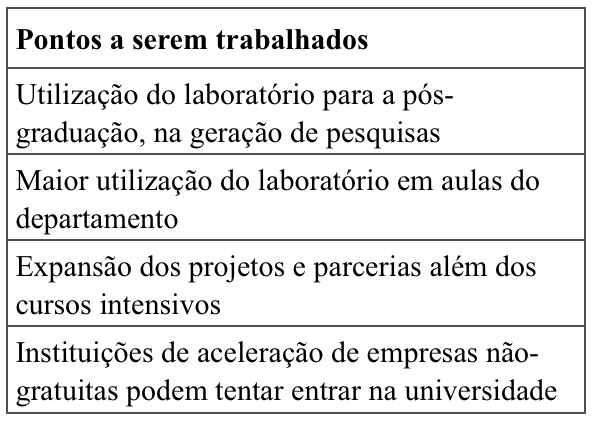
\includegraphics[scale=0.75]{img/pontosselecionadospassivos}}
\label{fig:pontosselecionadospassivos}
\caption* {Fonte: Elaborado pelo próprio autor}
\end{figure}

\item[Pontos levantados pelos cursistas] - Em relação aos pontos levantados sobre \textit{feedbacks} dos cursistas, será elaborado um relatório executivo com menor teor acadêmico porém mais detalhes diante das análises realizadas. Em relação aos cursos básicos, poderá ser feita uma segmentação dos \textit{feedbacks} por ano de realização do questionário ou por tipo de curso dado pelo laboratório. Já para os cursos intensivos, poderão ser explorados os pontos levantados do ponto de vista de cada grupo, incluindo a identificação de \enquote{frases de efeito} que poderiam ser utilizadas em um material de divulgação do curso. Não obstante, como esses pontos devem ser trabalhados quase que exclusivamente pela gestão da Samsung, serão levantadas questões a respeito de como desenvolver esses pontos, porém eles apresentam pouca prioridade para os fins deste trabalho.

\begin{figure}[H]
\caption{Pontos levantados pelos cursistas}
\centerline{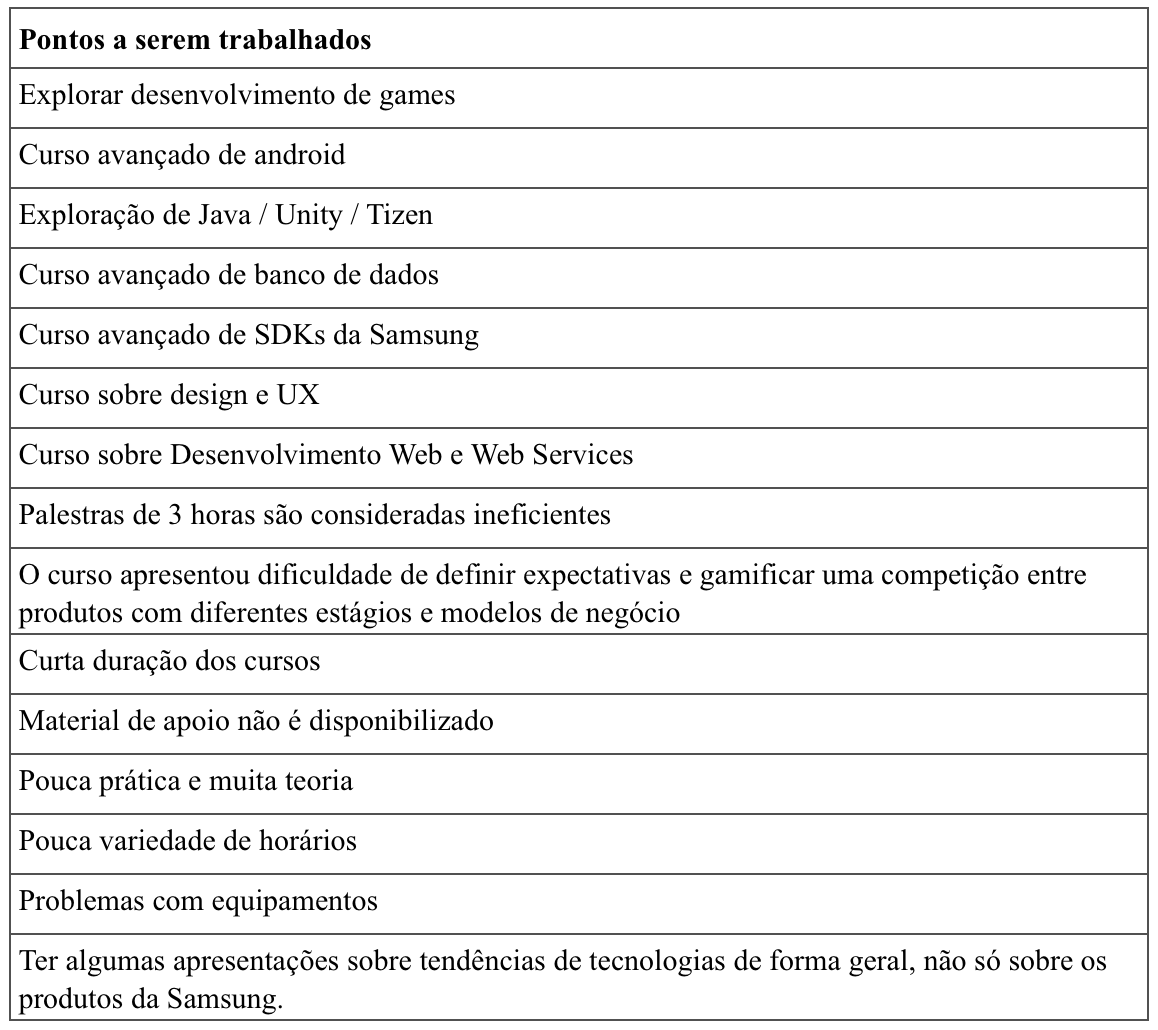
\includegraphics[scale=0.75]{img/pontosselecionadoscursistas}}
\label{fig:pontosselecionadoscursistas}
\caption* {Fonte: Elaborado pelo próprio autor}
\end{figure}

\item[Pontos considerados operacionais] - Os pontos operacionais são aqueles que podem ser corrigidos com alguma ação a ser tomada sem a necessidade de tomar algum decisão considerada estratégica pela gestão. Dentro desses pontos estão \enquote{Falta de conhecimento sobre os programas do laboratório}, \enquote{Falta de instruções sobre o processo de utilização} e \enquote{Falta de agenda pública com os compromissos do Ocean}. São pontos relevantes, e a gestão deverá fazer algo a respeito deles para maximizar o uso do laboratório pelos alunos.

\begin{figure}[H]
\caption{Pontos operacionais}
\centerline{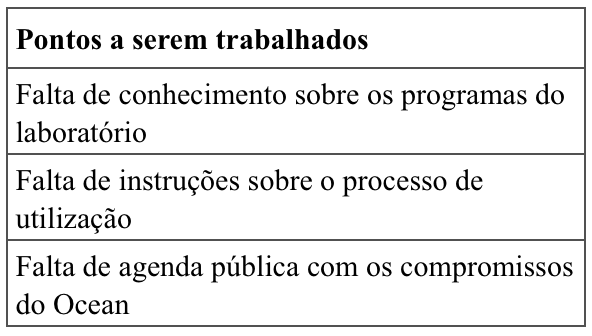
\includegraphics[scale=0.75]{img/pontosselecionadosoperacionais}}
\label{fig:pontosselecionadosoperacionais}
\caption* {Fonte: Elaborado pelo próprio autor}
\end{figure}

\item[Pontos estratégicos] - Os pontos considerados mais estratégicos são aqueles que podem ser desenvolvidos e transformados em projetos de curto, médio ou longo prazo, e têm potencial de trazer um impacto muito positivo para o Ocean.

\begin{figure}[H]
\caption{Pontos estratégicos}
\centerline{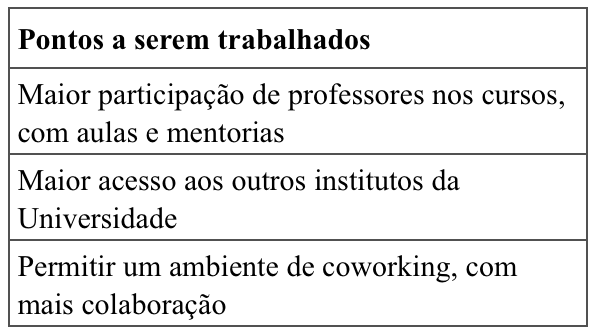
\includegraphics[scale=0.75]{img/pontosselecionadosestrategicos}}
\label{fig:pontosselecionadosestrategicos}
\caption* {Fonte: Elaborado pelo próprio autor}
\end{figure}

\end{description}

Definidas as categorias, foram definidos níveis de priorização para cada uma, juntamente com a gestão do laboratório Ocean. Foram atribuídas as notas 1, 3, 5 e 7 para as categorias, sendo a nota 1 os pontos com maior prioridade e o 7 os de menor prioridade.

\begin{figure}[H]
\caption{Priorização de pontos}
\centerline{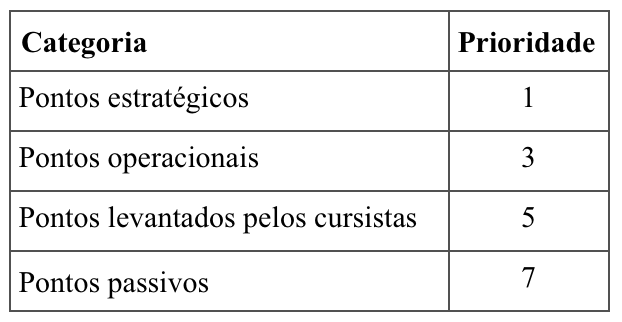
\includegraphics[scale=0.75]{img/priorizacao}}
\label{fig:priorizacao}
\caption* {Fonte: Elaborado pelo próprio autor}
\end{figure}

Devido ao maior impacto no posicionamento do Ocean dentro do ecossistema de inovação e empreendedorismo dentro do PRO, da Poli e da USP, foram priorizados os pontos estratégicos frente aos outros pontos levantados, seguido pelos pontos operacionais por serem fáceis de implementar e por terem um possível impacto positivo na experiência dos usuários do laboratório. Em seguida se encontrariam os pontos levantados pelos cursistas, pois envolvem um esforço maior de reavaliar as mudanças diante da estratégia de capacitação de difusão da marca utilizada pela Samsung, e por fim os pontos passivos que não possuem ação imediata a ser tomada diante dessas frentes.

\section{Exploração dos pontos prioritários}

Cada um dos pontos prioritários será explorado de tal forma a guiar a gestão do Ocean a tomar ações futuras diante desses pontos, simplificando o processo de estruturação do problema e identificação de possíveis soluções. Embora haja espaço para o desenvolvimento de propostas de solução completas, apenas foi proposto o ponto de partida de novos projetos.

\subsection{Maior participação de professores nos cursos}

Segundo a gestão do Ocean, a participação de professores nas frentes de ensino dos cursos enriqueceria o conteúdo transmitido, pois fornece uma base teórica que em si justifica grande parte dos métodos utilizados atualmente de forma empírica. Não obstante, a grande variedade de cursos superiores entre os participantes dos programas intensivos têm como consequência pessoas que têm bastante conhecimento sobre certas metodologias e outras que tiveram pouco ou nenhum  contato com as mesmas, o que dá espaço para um professor especialista reafirmar um assunto para os especialistas e abrir novos horizontes para os menos experientes. 

A Universidade de São Paulo possui grandes educadores em todos os seus institutos, e em especial o IME, FEA e as faculdades da Poli possuem professores especialistas em criação e desenvolvimento de produtos, inovação e empreendedorismo, que trariam muito conhecimento para os cursistas e para o programa. Entretanto, como a participação de professores nos cursos ainda não ocorre com muita frequência, seria prudente começar a intensificação desse tipo de parceria pelo PRO, pois se mantém a facilidade de comunicação entre o laboratório e o departamento, sem uma necessidade de modificar ou estruturar os processos atuais de funcionamento e comunicação do Ocean.

Considerando a grade de ensino da Engenharia de Produção da Poli, observa-se que muitas disciplinas possuem uma sinergia muito grande com a proposta de pré-aceleração de empresas do laboratório: 

\begin{description}
\item[Projeto Integrado de Sistemas de Produção] - tem como objetivo \enquote{Estabelecer uma ponte entre a formação acadêmica e o mundo profissional, com foco no planejamento, elaboração e implantação de projetos e novos empreendimentos}, e introduz muitos conceitos como planos de modelo de negócio - guiado principalmente pelo \textit{Canvas} - e fontes de captação de recursos, como \enquote{\textit{Venture Capitals}} e \enquote{\textit{Private Equities}}

\item[Projeto do Produto e Processo] - segmenta o processo de desenvolvimento de um produto em diversas etapas de validação, \enquote{Concepção do Produto}, \enquote{Avaliação do preço do produto}, \enquote{Desenvolvimento do Produto}, \enquote{Desenvolvimento dos Desenhos de Engenharia}, \enquote{Resolução do Processo}, \enquote{Sistema de informação e Layout}, \enquote{Viabilidade Comercial e Engenharia de Valor}

\item[Projeto, Processo e Gestão da Inovação] - discute como empresas devem se organizar para facilitar e fomentar a gestão da inovação para criar oportunidades de negócios, através da criação e acompanhamento de projetos-chave e da definição de proessos e KPIs para os seus principais objetivos.

\end{description}

Muitas outras disciplinas ainda apresentam conceitos interessantes que poderiam ser utilizados em um escopo menor do que o apresentado na disciplina, como a \enquote{Gestão de Projetos} e \enquote{Princípios de Marketing para Engenharia de Produção}, ilustrando a possível sinergia entre os professores do departamento e o laboratório Ocean através do conteúdo ensinado em aula para os alunos do PRO.

Embora toda essa sinergia evidencie o quanto os professores podem enriquecer os cursos do Ocean, ela não é suficiente para garantir uma maior participação de professores nos cursos, pois embora o laboratório seja de cogestão do PRO os cursos são geridos pela Samsung, o que traz algumas complicações para essa parceria. Os cursos normalmente possuem horário incompatível com a grade horária dos professores, o escopo do trabalho dos professores já está bem definido, e por ser um projeto inicial, não há muito investimento dos professores planejado com o laboratório. No entanto, sabe-se que por a Samsung ser uma empresa externa à universidade, a parceria com os docentes poderia ser facilitada através do financiamento de palestras, aulas e mentorias, o que é inexistente no momento.

Em conversa com Selber, gestor da unidade Ocean, foi discutida a possibilidade de financiamento dos professores, e a barreira existente para isso acontecer está na organização da Gestão Financeira da \textit{Samsung} diante dos recursos separados para a Lei da Informática. No formato atual, existe uma limitação no número de fornecedores ou prestadores de serviço que o laboratório pode contratar. Hoje, todas as contratações feitas pelo laboratório, entre consultorias externas, empresas de segurança e limpeza são realizadas diretamente através do laboratório. A remuneração de professores entraria como um novo fornecedor, porém os fornecedores atuais do departamento já atingiram a limitação imposta. Dessa forma, uma das maneiras de superar essa limitação seria centralizar a contratação de serviços em um fornecedor só, que por sua vez contrataria os demais.

Atualmente, os professores do PRO mantém o funcionamento da Fundação Vanzolini, instituição privada e sem fins lucrativos que tem como objetivo principal desenvolver e disseminar conhecimentos científicos e tecnológicos essenciais à Engenharia de Produção. A fundação fornece cursos à nível de MBA e pós-graduação ou certificações para empresas e órgãos públicos. Uma das alternativas para viabilizar a remuneração de professores seria centralizar a contratação de fornecedores através da Fundação Vanzolini, eliminando a limitação de fornecedores contratados pelo laboratório Ocean. A Gestão do PRO já está estudando a viabilização desse processo, que por sua vez facilitaria o financiamento de professores do Departamento a participarem dos cursos, enriquecendo o conteúdo passado aos cursistas.

\subsection{Maior acesso aos outros institutos da universidade}

O acesso ao laboratório discutido nesta seção pode ser visto através de duas frentes: uso do espaço do laboratório e inscrições nos cursos do programa. Em ambas as situações, a grande maioria dos alunos envolvidos vêm da Poli, devido à facilidade de divulgação via boca-a-boca dentro da faculdade.

Em relação ao uso do espaço, é muito difícil atrair pessoas de outros institutos ao laboratório apenas com sua infraestrutura, dada ao incômodo de locomoção entre departamentos dentro da Cidade Universitária. Alguns serviços externos e únicos, como o ambiente de \textit{coworking} discutido na próxima seção, seriam interessantes para atrair outros institutos a utilizarem o laboratório no dia-a-dia.

Já em relação às inscrições nos cursos oferecidos pelo programa, o Ocean depende muito de iniciativas de divulgação realizadas a partir do NEU. Entretanto, assim como o Ocean, o NEU também possui maior participação dentro da Poli, com alguns membros da Faculdade de Arquitetura e Urbanismo (FAU), e ainda está em fase de obter mais acesso aos outros institutos aos poucos, através de parcerias em projetos e \textit{workshops}. O laboratório Ocean poderia utilizar a mesma estratégia de aproximação utilizada pelo NEU para atingir outros institutos, utilizando as parcerias como canal de entrada e acesso aos estudantes do departamento.

Baseado nessa estratégia de buscar parcerias com outros departamentos, foram mapeados alguns dos principais grupos de inovação e empreendedorismo da universidade que a gestão do Ocean pode entrar em contato para possíveis parcerias na Figura \ref{fig:institutosuniversidade}. Todos esses grupos são facilmente acessíveis dentro da Cidade Universitária, com exceção do \textit{Habits} que se localiza dentro da USP Leste. Todos mantém projetos ativos e possuem um canal no \textit{facebook} de fácil acesso, permitindo um contato fácil com os membros de cada grupo.

\begin{figure}[H]
\caption{Grupos de Inovação e Empreendedorismo da Universidade}
\centerline{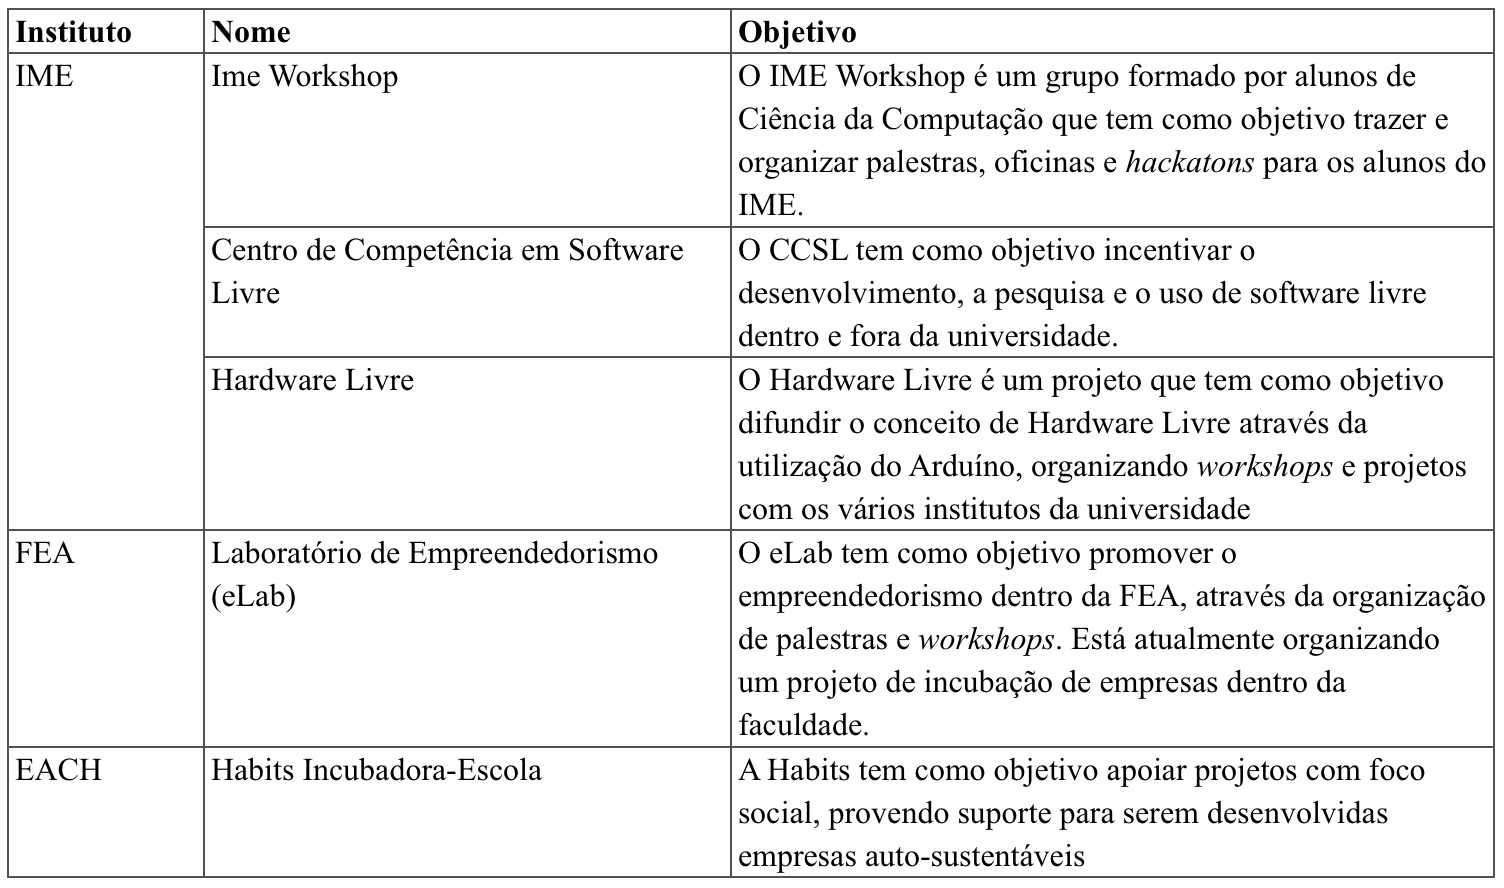
\includegraphics[scale=0.6]{img/institutosuniversidade}}
\label{fig:institutosuniversidade}
\caption* {Fonte: Elaborado pelo próprio autor}
\end{figure}

\subsection{Permitir um ambiente de \textit{coworking}, com mais colaboração}

A proposta de um ambiente de \textit{coworking} visa transformar o espaço do laboratório em um ambiente colaborativo de trabalho, intensificando ainda mais o ecossistema de inovação e empreendedorismo em que se encontra dentro do PRO. Dessa forma, o laboratório assumiria um papel bem diferente da biblioteca e do laboratório de informática do departamento, evitando redundâncias e deixando mais claro a função de cada um.

Atualmente, existem alguns modelos de espaços de \textit{coworking} muito interessantes em funcionamento hoje em dia, sendo a principal referência mundial o Google Campus, que abriu sua instalação em São Paulo este ano. O Campus possui mais 5 instalações ao redor do mundo, em Londres, Madrid, Seul,  Tel Aviv e Warsaw, e todas as instalações têm o mesmo propósito: \enquote{Ser um espaço para empreendedores}. Portanto, todas as unidades apresentam uma série de espaços para empreendedores ou interessados/envolvidos com empreendedorismo, desde que se inscrevam no programa preenchendo um formulário que descreve a sua relação com o empreendedorismo.

Um dos pontos mais bem avaliados pelos usuários do Google Campus de São Paulo é a presença de pessoas relacionadas com empreendedorismo em todos os níveis, desde desenvolvedores de \textit{software} que desejam empreender quanto investidores, mentores e até empreendedores de \textit{startups} que já estão em funcionamento. O grande movimento dessa variedade de pessoas dentro do Campus se deve principalmente aos seguintes fatores: 

\begin{description}
\item[Gratuidade] - Atualmente o campus possui reservado dois andares do prédio para o Google Café, com wi-fi gratuito, sem necessário agendamento prévio ou processo seletivo. Atua com uma proposta parecida ao \textit{Starbucks} ou até o Centro Cultural SP, em que é possível comprar alimentos e bebidas no estabelecimento, porém não é necessário para utilizar a infraestrutura do ambiente.

\item[Acessibilidade] - O Google Campus SP se localiza a duas quadras da Avenida Paulista e da estação de Metrô Brigadeiro, e possui um andar de estacionamento e um com bicicletários e vestiários, tornando o ambiente já bem localizado com facilidade de acesso.

\item[Palestras e Eventos] - O Google Campus ainda possui um auditório e um andar para a realização de eventos, gratuitos porém limitado ao número de inscritos. Os eventos podem ser organizados por qualquer pessoa ou empresa que deseja apresentar um conteúdo relevante para a comunidade empreendedora.

\item[Incubação de Empresas] - O Campus realiza uma incubação de empresas chamadas de residentes por um período de 6 meses. Nos quais elas recebem mentorias e têm acesso a palestras e um espaço de \textit{coworking} durante esse período.
\end{description}

Ao se comparar os pontos fortes do Google Campus com os do Ocean, mantidas as proporções de investimento realizado em cada um, é possível observar que, com exceção da incubação de empresas, todos os outros fatores também são oferecidos pelo Ocean. O laboratório oferece wifi e acesso aos equipamentos gratuitamente, com fácil acessibilidade para a comunidade uspiana, e sedia diversos eventos dentro de seu espaço. Embora não esteja trabalhando com a incubação de empresas atualmente, grande parte dos benefícios de uma incubação são cobertos pelo programa dos cursos intensivos do laboratório, como mentorias e palestras.

Portanto ao se comparar ambos ambientes, sendo o Google Campus a referência de espaço de \textit{coworking} em São Paulo, é possível observar que ambos atuam na mesma direção em relação ao fomento do empreendedorismo e do auxílio direto na formação de empresas. Partindo desse ponto de vista, seria justo assumir que a incubação de empresas favorece em muito ao estabelecimento de um espaço de \textit{coworking}, dado que funciona muito bem no Campus. Não obstante, seria muito interessante pensar na incubação de empresas como uma versão futura dos atuais cursos intensivos. Com a maior utilização do ambiente por empresas de verdade e o acesso aberto aos estudantes da universidade, poderia se instaurar um ambiente de colaboração mútua. Em relação à infraestrutura, o laboratório poderia utilizar metade da sala para a incubação, e a outra metade livre para uso de pessoas ou eventos. Algumas salas de reunião pequenas também seriam úteis para a realização de alguns \textit{brainstormings} e discussões.

Outro fator que colaboraria positivamente com um aumento de pessoas utilizando o laboratório como um espaço de \textit{coworking} seria o aumento do número de palestras e eventos apresentados no laboratório relacionados a temas de empreendedorismo. Essas palestras trariam empreendedores para o laboratório, que iria ganhando tração conforme mais palestras fossem sendo apresentadas.
